\documentclass{beamer}
\usepackage[utf8]{inputenc}

\usetheme{Madrid}
\usecolortheme{default}
\usepackage{amsmath,amssymb,amsfonts,amsthm}
\usepackage{txfonts}
\usepackage{tkz-euclide}
\usepackage{listings}
\usepackage{adjustbox}
\usepackage{array}
\usepackage{tabularx}
\usepackage{gvv}
\usepackage{lmodern}
\usepackage{circuitikz}
\usepackage{tikz}
\usepackage{graphicx}
\usepackage{mathtools}
\setbeamertemplate{page number in head/foot}[totalframenumber]

\usepackage{tcolorbox}
\tcbuselibrary{minted,breakable,xparse,skins}



\definecolor{bg}{gray}{0.95}
\DeclareTCBListing{mintedbox}{O{}m!O{}}{%
  breakable=true,
  listing engine=minted,
  listing only,
  minted language=#2,
  minted style=default,
  minted options={%
    linenos,
    gobble=0,
    breaklines=true,
    breakafter=,,
    fontsize=\small,
    numbersep=8pt,
    #1},
  boxsep=0pt,
  left skip=0pt,
  right skip=0pt,
  left=25pt,
  right=0pt,
  top=3pt,
  bottom=3pt,
  arc=5pt,
  leftrule=0pt,
  rightrule=0pt,
  bottomrule=2pt,
  toprule=2pt,
  colback=bg,
  colframe=orange!70,
  enhanced,
  overlay={%
    \begin{tcbclipinterior}
    \fill[orange!20!white] (frame.south west) rectangle ([xshift=20pt]frame.north west);
    \end{tcbclipinterior}},
  #3,
}
\lstset{
    language=C,
    basicstyle=\ttfamily\small,
    keywordstyle=\color{blue},
    stringstyle=\color{orange},
    commentstyle=\color{green!60!black},
    numbers=left,
    numberstyle=\tiny\color{gray},
    breaklines=true,
    showstringspaces=false,
}

\title 
{2.5.30}
\date{September 6, 2025}


\author 
{Vivek K Kumar - EE25BTECH11062}



\begin{document}


\frame{\titlepage}
\begin{frame}{Question}
If the two lines 
\begin{align}
    L_1 &: x=5, \frac{y}{3-\alpha} = \frac{z}{-2} \text{ and} \\
    L_2 &: x=2, \frac{y}{-1} = \frac{z}{2-\alpha}
\end{align}
are perpendicular, then the value of $\alpha$ is \underline{\hspace{0.1\columnwidth}}
\\
\end{frame}



\begin{frame}{Variables used}
\begin{table}[H]    
  \centering
  \begin{table}[h!]
    \centering
    \begin{tabular}{|c|c|}
        \hline
        Point & Coordinates \\
        \hline
	    $A$ & $\myvec{1\\-1}$ \\
	    $B$ & $\myvec{-4\\2k}$ \\
	    $C$ & $\myvec{-k\\-5}$ \\
        \hline
    \end{tabular}
    \caption{Vertices of $\triangle ABC$ before substituting $k$}
    \label{tab:triangle_k}
\end{table}

  \caption{Variables Used}
  \label{tab:1.6.12}
\end{table}

\end{frame}

\begin{frame}{Solution}

The lines can be represented as\\
\begin{align}
\vec{x} &= \myvec{5\\0\\0} + \kappa_1\vec{m_1}\\
           &= \myvec{5\\0\\0} + \kappa_1\myvec{0\\3-\alpha\\-2}
\end{align}
and 
\begin{align}
\vec{x} &= \myvec{2\\0\\0} + \kappa_2\vec{m_2}\\
           &= \myvec{2\\0\\0} + \kappa_2\myvec{0\\-1\\2-\alpha}
\end{align}

\end{frame}
\begin{frame}{Solution}
As the given lines are perpendicular, their direction vectors follow the relation: 
\begin{align}
    \vec{m_1}^T\vec{m_2} = 0 \\
    \myvec{0&3-\alpha&-2}\myvec{0\\-1\\2-\alpha} = 0\\
    3\alpha - 7 = 0\\
    \text{which gives } \alpha = \frac{7}{3}\\
    \text{and } \vec{m_1} = \myvec{0 \\ \frac{2}{3} \\ -2} , \vec{m_2} = \myvec{0 \\ -1 \\ \frac{-1}{3}}
\end{align}
\end{frame}

\begin{frame}[fragile]
    \frametitle{Python - Importing libraries and checking system}
    \begin{lstlisting}
import sys
import numpy as np
import numpy.linalg as LA
import matplotlib.pyplot as plt
import matplotlib.image as mpimg

from libs.line.funcs import *
from libs.triangle.funcs import *
from libs.conics.funcs import circ_gen

import subprocess
import shlex

print('Using termux?(y/n)')
y = input()
\end{lstlisting}
\end{frame}

\begin{frame}[fragile]
    \frametitle{Python - Checking if 2 lines are perpendicular}
    \begin{lstlisting}
m1 = np.array([0, 2/3, -2]).reshape(-1, 1)
r1 = np.array([5, 0, 0]).reshape(-1, 1)
m2 = np.array([0, -1, -1/3]).reshape(-1,1)
r2 = np.array([2, 0, 0]).reshape(-1, 1)
O = np.zeros(3).reshape(-1, 1)
if(m1.T@m2 == 0):
    print('The two lines are perpendicular')
else:
    print('The two lines are not perpendicular')
\end{lstlisting}
\end{frame}

\begin{frame}[fragile]
    \frametitle{Python - Generating points and plotting}
    \begin{lstlisting}
p_m1 = line_gen(r1-8*m1, r1+8*m1)
p_m2 = line_gen(r2-8*m2, r2+8*m2)

fig = plt.figure()
ax = fig.add_subplot(111, projection = '3d')

ax.plot(p_m1[0, :], p_m1[1, :], p_m1[2, :], label = 'Line L1')
ax.plot(p_m2[0, :], p_m2[1, :], p_m2[2, :], label = 'Line L2')
\end{lstlisting}
\end{frame}

\begin{frame}[fragile]
    \frametitle{Python - Labelling points}
    \begin{lstlisting}
ax.set_xlabel('$x$')
ax.set_ylabel('$y$')
ax.set_zlabel('$z$')
ax.legend(loc='best')
ax.grid(True) 
ax.axis('equal')
    \end{lstlisting}
\end{frame}

\begin{frame}[fragile]
    \frametitle{Python - Saving figure and opening it}
    \begin{lstlisting}
fig.savefig('../figs/fig.png')
print('Saved figure to ../figs/fig.png')

if(y == 'y'):
    subprocess.run(shlex.split('termux-open ../figs/fig.png'))
else:
    subprocess.run(["open",  "../figs/fig.png"])
    \end{lstlisting}
\end{frame}


\begin{frame}{Plot-Using only Python}
    \centering
    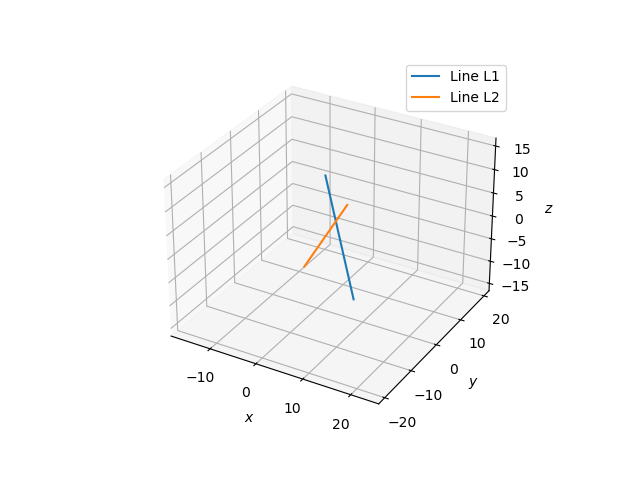
\includegraphics[width=\columnwidth, height=0.8\textheight, keepaspectratio]{../figs/fig.png}     
\end{frame}

\begin{frame}[fragile]
    \frametitle{C Code (0) - Importing libraries}

    \begin{lstlisting}
#include <stdio.h>
#include <stdlib.h>
#include <string.h>
#include <math.h>
#include <sys/socket.h>
#include <netinet/in.h>
#include <unistd.h>
#include "libs/matfun.h"
#include "libs/geofun.h"
    \end{lstlisting}
\end{frame}
\begin{frame}[fragile]
    \frametitle{C Code (1) - Function to Generate Points on a Line}

    \begin{lstlisting}

void point_gen(FILE *p_file, double **A, double **B, int rows, int cols, int npts){
    for(int i = 0; i <= npts; i++){
     double **output = Matadd(A, Matscale(Matsub(B, A, rows, cols), rows, cols, (double)i/npts), rows, cols);
     fprintf(p_file, "%lf, %lf, %lf\n", output[0][0], output[1][0], output[2][0]);
     freeMat(output, rows);
    }
}

    \end{lstlisting}
\end{frame}


\begin{frame}[fragile]
    \frametitle{C Code (2) - Function to write points b/w given point and origin to a file}

    \begin{lstlisting}
int check_perpendicularity(double **p1, double **p2, int m, int n);

int write_points(double x1, double y1, double z1, double x2, double y2, double z2, double x3, double y3, double z3, double x4, double y4, double z4, int npts){
    int m = 3;
    int n = 1;

    double **R = createMat(m, n);
    double **O = createMat(m, n);
    double **T = createMat(m, n);
    double **S = createMat(m, n);

    R[0][0] = x2;
    R[1][0] = y2;
    R[2][0] = z2;
    \end{lstlisting}
\end{frame}
\begin{frame}[fragile]
    \frametitle{C Code (2) - Function to write points b/w given point and origin to a file}

    \begin{lstlisting}
    O[0][0] = x1;
    O[1][0] = y1;
    O[2][0] = z1;

    T[0][0] = x4;
    T[1][0] = y4;
    T[2][0] = z4;

    S[0][0] = x3;
    S[1][0] = y3;
    S[2][0] = z3;
    \end{lstlisting}
\end{frame}

\begin{frame}[fragile]
    \frametitle{C Code (2) - Function to write points b/w given point and origin to a file}

    \begin{lstlisting}
    FILE *p_file;
    FILE *p_file_2;
    p_file = fopen("plot.dat", "w");
    p_file_2 = fopen("plot2.dat", "w");
    if(p_file == NULL || p_file_2 == NULL){
        printf("Error opening one of the data files\n");
    }
    point_gen(p_file, O, R, m, n, npts);
    point_gen(p_file_2, S, T, m, n, npts);
    int k = check_perpendicularity(Matsub(R, O, m, n), Matsub(T, S, m, n), m, n);
    freeMat(R, m);
    freeMat(O, m);
    freeMat(T, m);
    freeMat(S, m);
    fclose(p_file);
    fclose(p_file_2);
    return k;
}
    \end{lstlisting}
\end{frame}


\begin{frame}[fragile]
    \frametitle{C Code (3) - Checking Perpendicularity}

\begin{lstlisting}
int check_perpendicularity(double **p1, double **p2, int m, int n){
    return Matmul(transposeMat(p1, m, n), p2, n, m, n)[0][0];
}
\end{lstlisting}
\end{frame}

\begin{frame}[fragile]
    \frametitle{Python Code (0) - Importing libraries and checking system}
    \begin{lstlisting}
import numpy as np
import matplotlib.pyplot as plt
import ctypes
import os
import sys
import subprocess

print('Using termux? (y/n)')
termux = input()
\end{lstlisting}
\end{frame}

\begin{frame}[fragile]
    \frametitle{Python Code (1) - Using Shared Object}
    \begin{lstlisting}
lib_path = os.path.join(os.path.dirname(__file__), 'plot.so')
my_lib = ctypes.CDLL(lib_path)
my_lib.write_points.argtypes = [ctypes.c_double, ctypes.c_double, ctypes.c_double, ctypes.c_double, ctypes.c_double, ctypes.c_double, ctypes.c_double, ctypes.c_double, ctypes.c_double, ctypes.c_double, ctypes.c_double, ctypes.c_double, ctypes.c_int]
my_lib.write_points.restype = ctypes.c_int
r1 = np.array([5, 0, 0])
r2 = np.array([2, 0, 0])
m1 = np.array([0, 2/3, -2])
m2 = np.array([0, -1, -1/3])
p1 = r1 - 8*m1
p2 = r1 + 8*m1
p3 = r2 - 8*m2
p4 = r2 + 8*m2
k = my_lib.write_points(p1[0], p1[1], p1[2], p2[0], p2[1], p2[2], p3[0], p3[1], p3[2], p4[0], p4[1], p4[2], 20000)
\end{lstlisting}
\end{frame}

\begin{frame}[fragile]
    \frametitle{Python Code (2) - Loading points and checking perpendicularity}
    \begin{lstlisting}
if k == 0:
    print('The given lines are perpendicular')
else:
    print('The given lines are not perpendicular')

points = np.loadtxt('plot.dat', delimiter=',', usecols = (0,1, 2))
points2 = np.loadtxt('plot2.dat', delimiter=',', usecols = (0,1, 2))

x = points[:, 0]
y = points[:, 1]
z = points[:, 2]

x2 = points2[:, 0]
y2 = points2[:, 1]
z2 = points2[:, 2]
\end{lstlisting}
\end{frame}

\begin{frame}[fragile]
    \frametitle{Python Code (3) - Plotting points}
    \begin{lstlisting}
fig = plt.figure()
ax = fig.add_subplot(111, projection = '3d')
ax.plot(x, y, z, label = 'Line L1')
ax.plot(x2, y2, z2, label = 'Line L2')

ax.set_xlabel('$x$')
ax.set_ylabel('$y$')
ax.set_zlabel('$z$')
ax.legend(loc='best')
ax.grid() 
ax.axis('equal')

fig.savefig('../figs/fig2.png')
print('Saved figure to ../figs/fig2.png')
\end{lstlisting}
\end{frame}

\begin{frame}[fragile]
    \frametitle{Python Code (4) - Saving plot and opening it}
    \begin{lstlisting}
fig.savefig('../figs/fig2.png')
print('Saved figure to ../figs/fig2.png')

if(termux == 'y'):
    subprocess.run(shlex.split('termux-open ../figs/fig2.png'))
else:
    subprocess.run(["open",  "../figs/fig2.png"])
\end{lstlisting}
\end{frame}

\begin{frame}{Plot-Using Both C and Python}
    \centering
    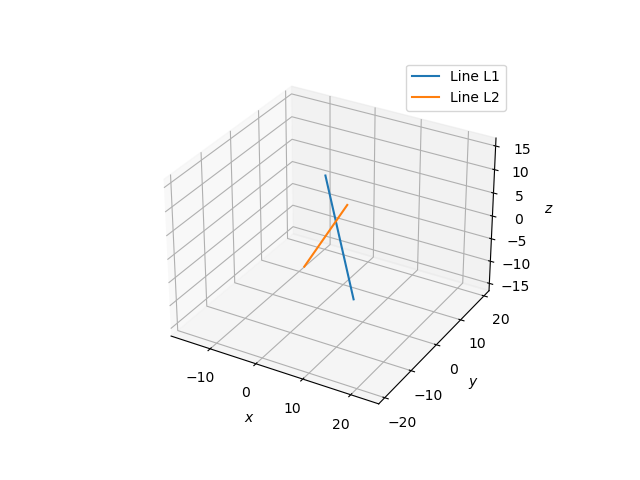
\includegraphics[width=\columnwidth, height=0.8\textheight, keepaspectratio]{../figs/fig2.png}     
\end{frame}

\end{document}